\documentclass[aspectratio=169,xcolor=dvipsnames, t]{beamer}
\usepackage{fontspec} % Allows using custom font. 
\usepackage{beamerthemeSimplePlusAIC} % Using the requested theme

\usepackage[utf8]{inputenc}
\usepackage[T1]{fontenc}
\usepackage[spanish]{babel}
\usepackage{hyperref}
\usepackage{listings}
\usepackage{xcolor}

\usepackage{polyglossia} % Para idioma
\usepackage{graphicx}
\usepackage{booktabs}
\usepackage{svg}
\usepackage{tikz}
\usepackage{makecell}
\usepackage{wrapfig}


\title[Vectorization]{Tokenización y Vectorización en NLP y LLMs} 
\subtitle{Conceptos, aplicaciones y ejemplos prácticos}

\author[Jorge]{ Inteligencia Artificial: Dr. Jorge Roa | Dra. Milagros Gutiérrez}
\institute[CIDISI]{CIDISI - UTN - FRSF}

\date{Mayo 2025} 

\begin{document}

\maketitlepage

% % Portada
% \begin{frame}
%     \titlepage
% \end{frame}

% Objetivos
\begin{frame}{Objetivos de la clase}
    \begin{itemize}
        \item Entender qué es la tokenización y vectorización y por qué son fundamentaled en NLP y LLMs.
        \item Conocer el concepto de word embeddings y su uso.
        \item Aprender cómo se vectorizan los prompts.
        \item Comprender la similaridad de vectores y su aplicación.
        \item Ver ejemplos prácticos.
        \item Introducción a los vector stores (bases de datos vectoriales).
    \end{itemize}
    \vspace{0.5cm}
    \textbf{Al final de la clase vas a poder explicar cómo los modelos de lenguaje entienden semánticamente el texto.}
\end{frame}

% ¿Qué es la tokenización?
\begin{frame}{¿Qué es la tokenización?}
    \begin{itemize}
        \item La \textbf{tokenización} es el proceso de dividir un texto en unidades más pequeñas llamadas \textbf{tokens}.
        \item Un token puede ser una palabra, subpalabra, carácter o símbolo.
        \item Ejemplo: ``\texttt{El perro duerme}'' $\rightarrow$ [``El'', ``perro'', ``duerme'']
    \end{itemize}
    \vspace{0.3cm}
    % \includegraphics[width=0.7\textwidth]{https://miro.medium.com/v2/resize:fit:1400/format:webp/1*8nG5QK1Qb6QwQKp1QK1gA.png}

\end{frame}

% % Tipos de tokenización
% \begin{frame}{Tipos de tokenización}
%     \begin{itemize}
%         \item \textbf{Por palabras:} cada palabra es un token.
%         \item \textbf{Por subpalabras:} se dividen palabras en partes más pequeñas (ej: ``jugando'' $\rightarrow$ ``jug'', ``ando'').
%         \item \textbf{Por caracteres:} cada letra o símbolo es un token.
%     \end{itemize}
%     \vspace{0.3cm}
%     % \includegraphics[width=0.8\textwidth]{https://jalammar.github.io/images/bert-tokenization-vocab.png}
% \end{frame}

% Tipos de tokenización (versión expandida)
\begin{frame}{Tipos de tokenización}
    \textbf{Existen diferentes formas de dividir el texto en tokens:}
    \vspace{0.3cm}
    \begin{itemize}
        \item \textbf{Tokenización por caracteres:}
        \begin{itemize}
            \item Cada letra o símbolo es un token.
            \item Ejemplo: \texttt{"gato"} $\rightarrow$ [``g'', ``a'', ``t'', ``o'']
            \item \textit{Ventaja:} máxima flexibilidad, nunca hay palabras desconocidas.
            \item \textit{Desventaja:} secuencias muy largas, pierde información semántica.
        \end{itemize}    
        \item \textbf{Tokenización por palabras:}
        \vspace{0.2cm}
        \begin{itemize}
            \item Cada palabra es un token.
            \item Ejemplo: ``\texttt{El perro juega}'' $\rightarrow$ [``El'', ``perro'', ``juega'']
            \item \textit{Ventaja:} simple y fácil de entender.
            \item \textit{Desventaja:} no maneja bien palabras desconocidas o errores de ortografía.
        \end{itemize}
        \vspace{0.2cm}
        \item \textbf{Tokenización por subpalabras:}
        \begin{itemize}
            \item Las palabras se dividen en partes más pequeñas (subpalabras o ``chunks'').
            \item Ejemplo: ``\texttt{jugando}'' $\rightarrow$ [``jug'', ``ando'']
            \item \textit{Ventaja:} permite manejar palabras nuevas, conjugaciones y errores.
            \item \textit{Desventaja:} los tokens pueden no tener significado por sí solos.
            % \item \textit{Ejemplo de tokenización BPE o WordPiece.}
        \end{itemize}
        \vspace{0.2cm}

    \end{itemize}
    \vspace{0.3cm}
    %\includegraphics[width=0.8\textwidth]{https://jalammar.github.io/images/bert-tokenization-vocab.png}
    
\end{frame}


% ¿Por qué es necesaria la tokenización?
\begin{frame}{¿Por qué es necesaria la tokenización?}
    \begin{itemize}
        \item Los modelos de IA no pueden trabajar directamente con texto crudo.
        \item La tokenización transforma el texto en una secuencia de unidades manejables.
        \item Permite manejar palabras desconocidas, errores de ortografía y diferentes idiomas.
        \item Es el primer paso antes de convertir el texto en vectores (embeddings).
    \end{itemize}
\end{frame}

% Tokenización y embeddings: el workflow
\begin{frame}{Tokenización y embeddings}
    \begin{enumerate}
        \item \textbf{Tokenización:} el texto se divide en tokens.
        \item \textbf{Mapeo a IDs:} cada token se convierte en un número (ID).
        \item \textbf{Embeddings:} cada ID se transforma en un vector numérico.
    \end{enumerate}
    \vspace{0.3cm}
    % \includegraphics[width=0.8\textwidth]{https://jalammar.github.io/images/transformer/tokenization.png}

\end{frame}



% Relación directa: tokens y embeddings
\begin{frame}{Relación directa: tokens y embeddings}
    \begin{itemize}
        \item Cada token tiene un embedding asociado en una tabla de embeddings.
        \item El modelo busca el vector correspondiente a cada token.
        \item Así, el texto se convierte en una secuencia de vectores que el LLM puede procesar.
        \item Ejercitación: \href{https://colab.research.google.com/drive/1LL-4FD0pkpl4zpbWYREUuspsDYNg0P3u\#scrollTo=0TRVc0xrzRWW}{Ir a Notebook}

    \end{itemize}
    \vspace{0.3cm}
    % \includegraphics[width=0.8\textwidth]{https://jalammar.github.io/images/transformer/transformer-inputs-embeddings.png}

\end{frame}




% ¿Qué es la vectorización?
\begin{frame}{¿Qué es la vectorización?}
    \begin{itemize}
        \item \textbf{Vectorizar} es transformar datos (por ejemplo, texto) en vectores numéricos.
        \item Los modelos de IA sólo pueden trabajar con números, no con palabras o frases.
        \item \textbf{Ejemplo:} la palabra "gato" podría representarse como el vector [0.3, 0.1, 0.65].
        \item \textbf{Analogia:} Es como traducir un idioma humano a un idioma que la computadora entiende.
    \end{itemize}
    
\end{frame}

% ¿Por qué es importante en NLP y LLM?
\begin{frame}{¿Por qué es importante en NLP y LLMs?}
    \begin{itemize}
        \item El texto es información no estructurada y ambigua.
        \item La vectorización permite:
        \begin{itemize}
            \item Procesar texto con modelos matemáticos.
            \item Comparar y buscar similitudes entre textos.
            \item Aprender relaciones semánticas y sintácticas.
        \end{itemize}
        \item Sin vectorización, los LLMs no podrían ``entender'' ni generar texto.
    \end{itemize}
    \vspace{0.3cm}
    
\end{frame}

% Ejemplo motivador: texto a números
\begin{frame}{Ejemplo motivador: de texto a números}
    \textbf{¿Cómo representamos la frase ``El perro juega''?}
    \begin{itemize}
        \item \textbf{One-hot encoding:} cada palabra es un vector con un 1 en la posición correspondiente y 0 en las demás.
        \item \textbf{Problema:} no captura relaciones entre palabras, y los vectores son muy grandes y dispersos.
    \end{itemize}
    \vspace{0.3cm}
    %\includegraphics[width=0.7\textwidth]{https://miro.medium.com/v2/resize:fit:1400/format:webp/1*8nG5QK1Qb6QwQKp1QK1gA.png}
    
    \vspace{0.2cm}
    \textit{Ejemplo: ``perro'' = [0, 1, 0, 0, 0, ...]}
\end{frame}

% Limitaciones del one-hot encoding
\begin{frame}{Limitaciones del one-hot encoding}
    \begin{itemize}
        \item No refleja similitud semántica: ``perro'' y ``gato'' son igual de diferentes que ``perro'' y ``auto''.
        \item Los vectores son muy grandes si el vocabulario es grande.
        \item No permite generalizar ni aprender relaciones entre palabras.
    \end{itemize}
    \vspace{0.3cm}
    \textbf{Solución:} usar \textbf{word embeddings}.
\end{frame}

% Word embeddings: ¿qué son y para qué sirven?
\begin{frame}{Word embeddings: ¿qué son y para qué sirven?}
    \begin{itemize}
        \item Son representaciones densas y continuas de palabras en un espacio vectorial de baja dimensión (por ejemplo, 300 dimensiones).
        \item Capturan relaciones semánticas y sintácticas entre palabras.
        \item Palabras con significados similares tienen vectores cercanos.
        \item Ejemplo: \texttt{king - man +  \( woman \approx queen \)}
        \item Modelos populares: Word2Vec, GloVe, FastText, embeddings de LLMs.
    \end{itemize}
    \vspace{0.2cm}
    \textit{Los embeddings se pueden aprender a partir de grandes corpus de texto.}
\end{frame}

% Ejemplo visual de word embeddings
\begin{frame}{Visualización de word embeddings}
    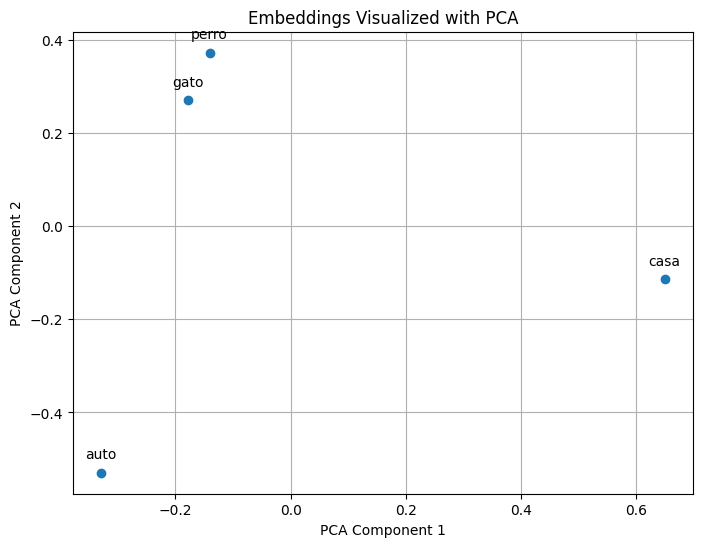
\includegraphics[width=0.7\textwidth]{figures/embeddings.png}
    
    \begin{itemize}
        \item Palabras con significados similares están cerca en el espacio vectorial.
        \item Relaciones como género, tiempo verbal, etc. se pueden representar como ``direcciones'' en el espacio.
    \end{itemize}
\end{frame}

% ¿Cómo se obtienen los word embeddings?
\begin{frame}{¿Cómo se obtienen los word embeddings?}
    \begin{itemize}
        \item Se entrenan modelos para que palabras que aparecen en contextos similares tengan vectores similares.
        \item \textbf{Ejemplo:} Word2Vec predice palabras vecinas en una oración.
        \item Los LLMs generan embeddings contextuales: el vector de una palabra depende de la frase.
        \item Visualización: \href{https://dash.gallery/dash-word-arithmetic/}{https://dash.gallery/dash-word-arithmetic/}

    \end{itemize}
    \vspace{0.2cm}
    \textit{Hoy en día, los embeddings de LLMs son el estándar para tareas avanzadas.}
\end{frame}

% Vectorización de prompts
\begin{frame}{Vectorización de prompts}
    \begin{itemize}
        \item Un \textbf{prompt} es el texto de entrada que le damos a un LLM.
        \item El modelo tokeniza el prompt (lo divide en palabras o subpalabras).
        \item Cada token se convierte en un vector (embedding).
        \item El LLM procesa la secuencia de vectores para generar una respuesta.
    \end{itemize}
    \vspace{0.3cm}
    %\includegraphics[width=0.8\textwidth]{https://jalammar.github.io/images/transformer/tokenization.png}
    
\end{frame}

% % Ejemplo visual: de texto a embeddings
% \begin{frame}{Ejemplo visual: de texto a embeddings}
%     \begin{itemize}
%         \item Texto: \texttt{El perro duerme}
%         \item Tokenización: [``El'', ``perro'', ``duerme'']
%         \item IDs: [101, 205, 304]
%         \item Embeddings: cada ID se transforma en un vector, por ejemplo:
%         \begin{itemize}
%             \item ``El'' $\rightarrow$ [0.12, 0.98, ...]
%             \item ``perro'' $\rightarrow$ [0.45, -0.22, ...]
%         \end{itemize}
%     \end{itemize}
%     \vspace{0.3cm}
%     % \includegraphics[width=0.8\textwidth]{https://jalammar.github.io/images/transformer/transformer-embeddings.png}

% \end{frame}

% Ejemplo: vectorización de un prompt
\begin{frame}{Ejemplo: vectorización de un prompt}
    \textbf{Prompt:} ¿Cuál es la capital de Argentina?"
    \begin{itemize}
        \item Tokenización: ["¿", ``Cuál'', ``es'', ``la'', ``capital'', ``de'', ``Argentina'', ``?'']
        \item Cada token se transforma en un vector numérico, por ejemplo:
        \begin{itemize}
            \item ``capital'' $\rightarrow$ [0.12, 0.98, -0.33, ...]
            \item ``Argentina'' $\rightarrow$ [0.45, -0.22, 0.67, ...]
        \end{itemize}
        \item El LLM procesa la secuencia de estos vectores para entender el significado del prompt.
    \end{itemize}
\end{frame}

% Similitud de vectores
\begin{frame}{Similitud de vectores}
    \begin{itemize}
        \item Permite medir cuán parecidos son dos textos o palabras.
        \item La métrica más usada es la \textbf{similitud de coseno}:
        \[
        \text{sim}(A, B) = \frac{A \cdot B}{\|A\| \|B\|}
        \]
        \item Valores cercanos a 1: muy similares; cercanos a 0: poco similares.
        \item Fundamental para tareas como búsqueda semántica y detección de duplicados.
    \end{itemize}
    \vspace{0.3cm}
    %\includegraphics[width=0.6\textwidth]{https://miro.medium.com/v2/resize:fit:1400/format:webp/1*ZpT1gkK1Qb6QwQKp1QK1gA.png}
    
\end{frame}

% % Ejemplo visual de similitud
% \begin{frame}{Ejemplo visual: similitud de coseno}
%     %\includegraphics[width=0.7\textwidth]{https://www.sciencedirect.com/science/article/pii/S1877050921001246/gr1.jpg}
    
%     \begin{itemize}
%         \item El ángulo entre los vectores determina la similitud.
%         \item Si el ángulo es pequeño, los vectores son similares.
%     \end{itemize}
% \end{frame}

% % Ejemplo práctico en PyTorch
% \begin{frame}[fragile]{Ejemplo práctico: word embeddings y similitud en PyTorch}
%     \textbf{Vectorizando palabras y calculando similitud de coseno}
%     \begin{lstlisting}[language=Python]
% import torch
% import torch.nn.functional as F

% # Supongamos que estos son embeddings de palabras
% perro = torch.tensor([0.2, 0.1, 0.7])
% gato = torch.tensor([0.3, 0.1, 0.65])
% auto = torch.tensor([0.9, 0.1, 0.1])

% # Similitud de coseno entre "perro" y "gato"
% sim_perro_gato = F.cosine_similarity(perro, gato, dim=0)
% print("Similitud perro-gato:", sim_perro_gato.item())

% # Similitud entre "perro" y "auto"
% sim_perro_auto = F.cosine_similarity(perro, auto, dim=0)
% print("Similitud perro-auto:", sim_perro_auto.item())
%     \end{lstlisting}
%     \textit{En general, palabras con significado similar tienen mayor similitud.}
% \end{frame}

% % Ejemplo práctico: vectorización de frases
% \begin{frame}[fragile]{Ejemplo práctico: vectorización de frases}
%     \textbf{Supongamos que tenemos dos frases:}
%     \begin{itemize}
%         \item ``El perro duerme''
%         \item ``Un gato descansa''
%     \end{itemize}
%     \textbf{¿Cómo comparamos su significado?}
%     \begin{lstlisting}[language=Python]
% # Embeddings promedio de las palabras de cada frase
% frase1 = torch.mean(torch.stack([perro, torch.tensor([0.1,0.2,0.1]), torch.tensor([0.3,0.3,0.4])]), dim=0)
% frase2 = torch.mean(torch.stack([gato, torch.tensor([0.05,0.2,0.1]), torch.tensor([0.25,0.3,0.45])]), dim=0)

% sim_frases = F.cosine_similarity(frase1, frase2, dim=0)
% print("Similitud entre frases:", sim_frases.item())
%     \end{lstlisting}
%     \textit{Así se puede comparar el significado de frases completas.}
% \end{frame}

% Vector stores
\begin{frame}{¿Qué es un vector store?}
    \begin{itemize}
        \item Es una base de datos optimizada para almacenar y buscar vectores.
        \item Permite búsquedas semánticas: encontrar textos similares a un prompt.
        \item Ejemplos: FAISS, ChromaDB, Milvus, Pinecone.
        \item Muy usado en sistemas de retrieval-augmented generation (RAG) con LLMs.
        \item \textbf{Ventaja:} permite búsquedas rápidas en millones de documentos.
    \end{itemize}
    \vspace{0.3cm}
    %\includegraphics[width=0.7\textwidth]{https://miro.medium.com/v2/resize:fit:1400/format:webp/1*ZpT1gkK1Qb6QwQKp1QK1gA.png}
    
\end{frame}

% Ejemplo de uso de vector store
\begin{frame}{Ejemplo de uso de vector store}
    \begin{itemize}
        \item \textbf{Caso:} buscador de preguntas frecuentes (FAQ).
        \item Se vectorizan todas las preguntas y se almacenan en un vector store.
        \item Cuando un usuario hace una pregunta, se vectoriza el prompt y se busca la pregunta más similar.
        \item \textbf{Ventaja:} encuentra respuestas aunque la pregunta no sea exactamente igual.
    \end{itemize}
    \vspace{0.3cm}
    %\includegraphics[width=0.7\textwidth]{https://miro.medium.com/v2/resize:fit:1400/format:webp/1*ZpT1gkK1Qb6QwQKp1QK1gA.png}
    
\end{frame}

% Aplicaciones
\begin{frame}{Aplicaciones de la vectorización}
    \begin{itemize}
        \item Búsqueda semántica de documentos: encontrar textos relevantes aunque no coincidan exactamente las palabras.
        \item Clasificación de texto: spam, sentimiento, temas, etc.
        \item Detección de similitud y plagio.
        \item Sistemas de recomendación de contenido.
        \item Retrieval-augmented generation (RAG) en LLMs: combinar búsqueda y generación de texto.
        \item Chatbots inteligentes y asistentes virtuales.
   
    \end{itemize}
\end{frame}

% Ejercitación
\begin{frame}{Ejercitación}
    \begin{itemize}
        \item Vectorización manual: \href{https://colab.research.google.com/drive/1lWR99IhnOiHOnKlOUWuQlBL8pcHY5PD5\#scrollTo=Fx-0HLDUK_wM}{Ir a Notebook}
        \item Vectorización automática: \href{https://colab.research.google.com/drive/10Ds4ZQdVTWCi_ZxqktKeMYL76MM1uiXm\#scrollTo=0HSh_TkDow-W}{Ir a Notebook}        
        \item Ejemplo con base de datos vectorial: \href{https://colab.research.google.com/drive/1-gbWhC5NyxAoB8Rd9KQm8k4eGlmw4GKL\#scrollTo=FR7XgQ_RwSY1}{Ir a Notebook}   
    \end{itemize}
\end{frame}

% Resumen
\begin{frame}{Resumen}
    \begin{itemize}
        \item La vectorización es clave para que los modelos de NLP y LLMs procesen texto.
        \item Los word embeddings permiten representar palabras y textos en forma numérica y semántica.
        \item La similitud de vectores es fundamental para comparar textos y buscar información relevante.
        \item Los vector stores permiten búsquedas eficientes y semánticas en grandes volúmenes de datos.
    \end{itemize}
    \vspace{0.3cm}
    \textbf{¡La vectorización es el puente entre el lenguaje humano y la inteligencia artificial!}
\end{frame}

% % Preguntas para los estudiantes
% \begin{frame}{Preguntas}
%     \begin{itemize}
%         \item ¿Por qué no podemos usar texto directamente en un modelo de deep learning?
%         \item ¿Qué ventajas tienen los word embeddings sobre el one-hot encoding?
%         \item ¿Cómo podrías usar la similitud de vectores en una aplicación real?
%         \item ¿Qué rol cumplen los vector stores en sistemas modernos con LLMs?
%         \item ¿Qué limitaciones pueden tener los embeddings?
%     \end{itemize}
% \end{frame}

% % Slide 1: ¿Qué es un vector en IA?
% \begin{frame}{¿Qué es un vector en IA?}
%     \begin{itemize}
%         \item Un \textbf{vector} es una lista ordenada de números.
%         \item En IA, los vectores representan información de manera numérica.
%         \item Ejemplo: $[0.2, 0.5, -0.1, 0.8]$
%         \item Los modelos de deep learning sólo pueden trabajar con números, no con palabras.
%     \end{itemize}
%     \vspace{0.3cm}
%     %\includegraphics[width=0.6\textwidth]{https://upload.wikimedia.org/wikipedia/commons/9/9e/Vector_space.svg}
    
%     \tiny{Fuente: Wikipedia}
% \end{frame}

% % Slide 2: ¿Qué es un embedding?
% \begin{frame}{¿Qué es un embedding?}
%     \begin{itemize}
%         \item Un \textbf{embedding} es una representación vectorial densa de una palabra, frase o documento.
%         \item Los embeddings capturan el significado y las relaciones semánticas entre palabras.
%         \item Ejemplo: la palabra "perro" puede representarse como un vector de 384 números.
%         \item Palabras con significados similares tienen embeddings (vectores) cercanos.
%     \end{itemize}
%     \vspace{0.3cm}
%     %\includegraphics[width=0.7\textwidth]{https://jalammar.github.io/images/word2vec/word2vec-king-queen.png}
    
%     \tiny{Fuente: jalammar.github.io}
% \end{frame}

% % Slide 3: ¿Cómo usan los LLMs los embeddings?
% \begin{frame}{¿Cómo usan los LLMs los embeddings?}
%     \begin{itemize}
%         \item Los LLMs convierten cada palabra o token del texto en un vector (embedding).
%         \item Estos vectores son la entrada al modelo y permiten que la red neuronal procese el texto.
%         \item Los embeddings permiten que el modelo entienda similitudes, contexto y relaciones.
%     \end{itemize}
%     \vspace{0.3cm}
%     %\includegraphics[width=0.8\textwidth]{https://jalammar.github.io/images/transformer/tokenization.png}
    
%     \tiny{Fuente: jalammar.github.io}
% \end{frame}

% % Slide 4: Analogía visual
% \begin{frame}{Analogía visual: palabras como puntos en el espacio}
%     \begin{itemize}
%         \item Imaginá que cada palabra es un punto en un espacio de muchas dimensiones.
%         \item Palabras con significados parecidos están cerca; palabras diferentes, lejos.
%         \item Así, el modelo puede “medir” similitud y contexto usando distancias entre vectores.
%     \end{itemize}
%     \vspace{0.3cm}
%     %\includegraphics[width=0.7\textwidth]{https://jalammar.github.io/images/word2vec/word2vec-tsne.png}
    
%     \tiny{Fuente: jalammar.github.io}
% \end{frame}

% % Slide 5: Ejemplo concreto en LLMs
% \begin{frame}{Ejemplo concreto en LLMs}
%     \begin{itemize}
%         \item Prompt: \texttt{"El perro duerme en la casa"}
%         \item Tokenización: ["El", "perro", "duerme", "en", "la", "casa"]
%         \item Cada token se convierte en un vector (embedding).
%         \item El LLM procesa la secuencia de vectores para generar una respuesta.
%     \end{itemize}
%     \vspace{0.3cm}
%     %\includegraphics[width=0.8\textwidth]{https://jalammar.github.io/images/transformer/transformer-embeddings.png}
    
%     \tiny{Fuente: jalammar.github.io}
% \end{frame}

% % Slide 6: Resumen visual
% \begin{frame}{Resumen visual}
%     \begin{itemize}
%         \item \textbf{Texto $\rightarrow$ Tokenización $\rightarrow$ Embeddings (vectores) $\rightarrow$ LLM}
%         \item Los vectores (embeddings) son el puente entre el lenguaje humano y la inteligencia artificial.
%         \item Permiten que los LLMs “entiendan” y generen texto de manera inteligente.
%     \end{itemize}
%     \vspace{0.3cm}
%     %\includegraphics[width=0.8\textwidth]{https://jalammar.github.io/images/transformer/transformer-inputs-embeddings.png}
    
%     \tiny{Fuente: jalammar.github.io}
% \end{frame}

\end{document}